% =========================================================================
% SciPost LaTeX template
% Version 1e (2017-10-31)
% =========================================================================

% For submitting a paper to SciPost Physics: 
\documentclass[submission, Phys]{SciPost}

\usepackage{multirow}
 \usepackage[utf8]{inputenc} 

\linenumbers

\begin{document}

% title
\begin{center}{\Large \textbf{
  Constraining new physics from Higgs measurements with\\[1mm] Lilith: update to LHC Run~2 results}}\end{center}

% Authors; mark the corresponding author with a superscript *.
\begin{center}
Thi Nhung Dao\textsuperscript{1},
Sabine Kraml\textsuperscript{2*},
Duc Ninh Le\textsuperscript{1},
Loc Tran Quang\textsuperscript{1}
\end{center}

% Affiliations
\begin{center}
{\bf 1} Institute For Interdisciplinary Research in Science and Education, ICISE,\\ 590000, Quy Nhon, Vietnam\\
{\bf 2} Laboratoire de Physique Subatomique et de Cosmologie, Universit\'e Grenoble-Alpes,\\ CNRS/IN2P3, 53 Avenue des Martyrs, F-38026 Grenoble, France\\
% email address of corresponding author
* sabine.kraml@lpsc.in2p3.fr
\end{center}

\begin{center}
\today
\end{center}

% For convenience during refereeing: line numbers
%\linenumbers

\section*{Abstract}
{\bf
Lilith is public python library for constraining new physics from Higgs signal strength measurements. 
We here present version 2.0 of Lilith together with an updated database which includes the full set 
of ATLAS and CMS Run~2 Higgs results for 36~fb$^{-1}$.  
Both the code and the XML database where extended from the ordinary Gaussian approximation employed in 
Lilith-1.1 to using variable Gaussian and Poisson distributions.  Moreover, Lilith can now make use of correlation 
matrices  of arbitrary dimension. 
We provide detailed validations of the implemented experimental results as well as 
a status of global fits for {\it i)} reduced Higgs couplings and {\it ii)} Two-Higgs-doublet models of Type-I and Type-II. 
Lilith-2.0 is available on GitHub and ready to be used to constrain a wide class of new physics scenarios.}


% include a table of contents if paper is longer than 6 pages
%\vspace{10pt}
%\noindent\rule{\textwidth}{1pt}
%\tableofcontents\thispagestyle{fancy}
%\noindent\rule{\textwidth}{1pt}
%\vspace{10pt}


%===================================================================================
\section{Introduction} \label{sec:intro}
%===================================================================================

Introduce Higgs couplings fits and  {\tt Lilith}~\cite{Bernon:2015hsa} .......  \\\
...........\\
...........\\
...........\\
...........\\
...........\\
...........\\


%%% Extended XML format %%%
\clearpage
%===================================================================================
\section{Extended XML format} \label{sec:xml}
%===================================================================================

In the Lilith database, every single experimental result is stored in a different XML file. 
The original input formats from~\cite{Bernon:2015hsa} are 
\begin{itemize} 
\item 1D intervals: best fit with $1\sigma$ errors; 
\item 2D likelihood contours: best fit, confidence level and parameters a, b, c which parametrize the inverse of the covariance matrix;
\item full likelihood information as 1D or 2D grids of $-2\log L$.
\end{itemize}
For a detailed discussion and description of the XML format, we refer the reader to the original Lilith manual~\cite{Bernon:2015hsa}. 
Here we just note that the first two options, 1D intervals and 2D likelihood contours, rely on an ordinary Gaussian approximation, 
which does not always describe the experimental data (i.e.\ the true likelihood) very well. 
Full 2D likelihood grids would be ideal but are rarely available.\footnote{We note that \cite{Boudjema:2013qla} strongly advocated 
the publication of full likelihood grids in 2 or more dimensions but unfortunately this wasn't followed up by the experimental collaborations.} 
We have therefore extended the XML format and fitting procedure in Lilith to include 
\begin{itemize} 
\item Gaussian distributions of variable width (``variable Gaussian'') and 
\item generalized Poisson distributions. 
\end{itemize}
For 1D and 2D data, the format follows the structure defined in \cite{Bernon:2015hsa}. The only difference is setting {\tt type="vn"} for a variable Gaussian and
{\tt type="p"} for a Poisson distribution in the {\tt <expmu>} tag. % (with {\tt dim="1"} for 1D and {\tt dim="2"} for 2D as before). 
The computation of the likelihood in {\tt computelikelihood.py} then follows Section~3.6 ``Variable Gaussian (2)'' of \cite{Barlow:2004wg}. 
Poisson distribution according to Section~3.4 ``Generalised Poisson'', eq.~(10a), of \cite{Barlow:2004wg}. 

This also now works for 2D data with a correlation.  
Taking the ATLAS result for $\mu(VBF, ZZ)$ and $\mu(ggH, ZZ)$ with correlation $\rho=-0.41$ from HIGG-2016-22 as an example:

\begin{verbatim}
<expmu decay="ZZ" dim="2" type="vn">
  <experiment>ATLAS</experiment>
  <source type="published">HIGG-2016-22</source>
  <sqrts>13</sqrts>
  <mass>125.09</mass>
  <CL>68\%</CL>  <!-- optional -->

  <eff axis="x" prod="VBF">1.0</eff>
  <eff axis="y" prod="ggH">1.0</eff>

  <bestfit>
    <x>4.0</x>
    <y>1.11</y>
  </bestfit>
 
  <param>
    <uncertainty axis="x" side="left">-1.46</uncertainty>
    <uncertainty axis="x" side="right">+1.75</uncertainty>
    <uncertainty axis="y" side="left">-0.21</uncertainty>
    <uncertainty axis="y" side="right">+0.23</uncertainty>
    <correlation>-0.41</correlation>
  </param>
</expmu>
\end{verbatim}

\noindent
Here, the {\tt <bestfit>} tag specifies the location of the best-fit point in the ({\tt x,y}) plane. 
The {\tt <uncertainty>} tags contain the left (negative) and right (positive) $1\sigma$ errors for the {\tt x} and {\tt y} axes. 
The {\tt <correlation>} tag specifies the correlation between {\tt x} and {\tt y}. 
The computation of the likelihood again follows Section~3.6 ``Variable Gaussian (2)'' of \cite{Barlow:2004wg}. 
Same for Poisson distribution, just setting {\tt type="p"}.

\subsection{Covariance matrices for ${\rm dim}>2$}



%%% Likelihood %%%
\clearpage
%===================================================================================
\section{Likelihood calculation} \label{sec:likelihood}
%===================================================================================
\newcommand{\lilith}{{\tt Lilith} }
\newcommand{\logL}{{ -2\log L } }
\newcommand{\XML}{ {\tt XML}}
\newcommand{\beq}{\begin{eqnarray}} 
\newcommand{\eeq}{\end{eqnarray}} 

\newcommand{\be}{\begin{equation}} 
\newcommand{\ee}{\end{equation}} 

\newcommand{\bpmatrix}{\begin{pmatrix}}
\newcommand{\epmatrix}{\end{pmatrix}}
\newcommand{\ba}{\begin{array}}
\newcommand{\ea}{\end{array}}
\newcommand{\braket}[1]{\left(#1\right)}
\newcommand{\sbraket}[1]{\left[#1\right]}
\newcommand{\bmu}{\bm{\mu}}
\newcommand{\hbmu}{\hat{\bm{\mu}}}
\newcommand{\diag}{\text{diag}}
\newcommand{\nhung}{\color{blue}}

The statistic procedure used in \lilith was described in details in ~\cite{Bernon:2015hsa}. 
The main quantity given as an output 
is the  $\logL$ which is computed according to the four different types of experimental data: 1D interval, 1D full,
2D contour, 2D full. Except for the full profile likelihoods, the $\logL$ values are computed using the ordinary Gaussian
distribution approximation. Since we have found that this assumption does not describe very well data in many cases, therefore
 we have added the  variable Gaussian and generalised Poison distributions. We have also extended the code to include the multi-dimensional data. In this section we present in details
how the  $\logL$ quantities are computed according to the two distribution approximations. For the old implementation of the  ordinary Gaussian distribution in \lilith
we refer the reader to ~\cite{Bernon:2015hsa}.
In the code, computations of $\logL$  are implemented in {\tt computelikelihood.py}.

%\noindent
%\subsection*{The ordinary Gaussian distribution}
%We have kept the old implementation of the  ordinary Gaussian distribution in \lilith, where the $\logL$ as function of 
%the single  signal strength $\mu$ in the 1D interval case reads ~\cite{Bernon:2015hsa}
%\be \logL(\mu) =  \begin{cases} 
%\braket{\frac{\mu - \hat\mu }{\sigma^-}}^2~~\text{if}~~\mu < \hat\mu,\\
% \braket{\frac{\mu - \hat\mu }{\sigma^+}}^2~~\text{if}~~\mu > \hat\mu,
%\end{cases}\ee
%where $\hat\mu$ denotes the best-fit signal strength, and $\sigma^-$ and $\sigma^+$ are the left and right uncertainties at 68\%
%CL, respectively. Note that $\hat\mu, \sigma^-,\sigma^+$ are taken directly from experimental papers. 
%For the two dimensional contour data of the two signal strengths $\mu_X,\mu_Y$, one has to digitize the contour lines at 68\% or 95\% CL.  Those 
%digitization data will be used to fit for the best fit point $ \hbmu=(\hat\mu_X, \hat\mu_Y)^T$ and the elements $a,b,c$ of the inverse of 
%covariance matrix, $C^{-1}$, assuming that the contour line is ellipse like. 
%In general, the fitted best fit point is not the same as the given best fit point since the contour line is not a 
%perfect ellipse. Those fitted parameters are then used to compute the $\logL$ of the two signal strengths $\bmu = ( \mu_X,
%\mu_Y)^T$  as
%\be \logL(\bmu) = (\bmu - \hbmu)^T C^{-1} (\bmu - \hbmu )  \quad \text{with}\quad C^{-1}=\bpmatrix a & b\\ b& c \epmatrix.\ee
 

\noindent
\subsection*{The variable Gaussian distribution}
As shown in \cite{Barlow:2004wg}, variable Gaussian distribution is one of good approximations to deal with 
asymmetric uncertainties. We apply the  ``Variable Gaussian (2)''  in  Section~3.6 of \cite{Barlow:2004wg}. 
In the 1D interval case, the likelihood is given by
\be \logL(\mu) =\frac{ \braket{\mu - \hat\mu }^2 }{\sigma^+\sigma^- + (\sigma^+ -\sigma^-)(\mu -\hat\mu)},\ee
where $\hat\mu$ denotes the best-fit signal strength, and $\sigma^-$ and $\sigma^+$ are the left and right uncertainties at 68\%
CL, respectively. Note that $\hat\mu, \sigma^-,\sigma^+$ are taken directly from experimental papers or fitted
if they are not given explicitly. If not stated otherwise, these notations are used for the entire section. 
The ordinary Gaussian distribution is obtained with  $\sigma^+ =\sigma^-$. The likelihood using variable Gaussian
however has a singularity point  at 
\be \mu= \hat\mu - \frac{\sigma^+\sigma^-}{\sigma^+ -\sigma^-}.\ee
This may happens if the values of reduced couplings may be two large and unphysical.
 In the case
of $n$ dimension data ($n>1$), we use the $n\times n$ correlation matrix  given by the experimental collaboration, if it is available,
together with the best fit points and the left and right uncertainties at 68\% CL.
Especially when data are given in terms of two dimensional contour plots, we can use also variable Gaussian to fit for the correlation and the best fit point and their uncertainties at 68 \% CL, if they are not given explicitly by the experimental collaboration. For the $n$ dimensional signal strength vector $\bmu = (\mu_1,\ldots,\mu_n)$, the likelihood reads
\be \logL(\bmu)= (\bmu - \hbmu)^T C^{-1} (\bmu - \hbmu ), \ee
where the best fit point $\hbmu = (\hat\mu_1,\ldots,\hat\mu_n)$ and the covariance matrix is constructed from the correlation matrix 
$\rho$ as
\be C = \bm{\Sigma}(\bmu).\rho.\bm{\Sigma}(\bmu) ,\quad \bm{\Sigma}(\bmu) =\diag (\Sigma_1, \ldots, \Sigma_n) \ee
with
\be \Sigma_i = \sqrt{\sigma^+_i\sigma_i^- + (\sigma^+_i-\sigma_i^-) (\mu_i - \hat\mu_i)}, \quad i =1,\ldots,n.\ee
Here the $\sigma^-_i$ and $\sigma^+_i$ are the left and right uncertainties at 68\% CL of the $i$th combination of production and decay channel, respectively. For the multi-dimensional data in the ordinary Gaussian distribution, the relation between covariance matrix and the correlation matrix becomes
\be C = \frac 14 [\bm{\sigma^+}+\bm{\sigma}^-]. \rho.[\bm{\sigma^+}+\bm{\sigma}^-], \ee
where $\bm{\sigma^+}=\diag(\sigma_1^+, \ldots,\sigma_n^+)$ and $\bm{\sigma^-}=\diag(\sigma_1^-, \ldots,\sigma_n^-)$.
\noindent
\subsection*{The generalised Poison distribution}
We apply the generalised Poison distribution for one and two dimensional data. For the one dimensional data, the likelihood is implemented according to ``Generalised Poisson'' of \cite{Barlow:2004wg},
\be  \log L(\mu) = -\nu\gamma(\mu-\hat\mu) + \nu\log\sbraket{1+\gamma\braket{\mu-\hat\mu}},\ee
where $\gamma$ and $\nu$ are solved numerically from the following equations
\be \frac{1- \gamma \sigma^-}{1+ \gamma \sigma^+} = e^{-\gamma(\sigma^+ + \sigma^-)}, \quad
 \nu = \frac{1}{2(\gamma \sigma^+ - \log (1+ \gamma\sigma^+))}. \label{eq:posonnugamma}\ee
For the two dimensional data,  we use the conditioning bivariate Poison distribution described in ~\cite{Berkhout:2004},
 that has no restriction on the sign and magnitude of the correlation $\rho$.  The joint distribution is a product of 
a marginal and a conditional distribution. The decision of which channel belongs to the marginal
or the conditional distribution is based on the validation plots. To illustrate our formulae,  
we assume that the data of the channel $X$ follows the marginal distribution
while data of  the channel $Y$ belongs to the conditional distribution. The joint log-likelihood is the the sum of 
the marginal and conditional log-likelihoods
\be \log L(\mu_X,\mu_Y) =  \log L(\mu_X)  +\log L(\mu_Y|\mu_X) ,\ee
where the marginal likelihood for the channel $X$ is given by
\be  \log L(\mu_X) =-\nu_X\gamma_X(\mu_X-\hat\mu_X) + \nu_X\log\sbraket{1+\gamma_X\braket{\mu_X-\hat\mu_X}},\ee
and the conditional likelihood for the channel $Y$ given the channel $X$
\be \log L(\mu_Y|\mu_X) = f(\mu_X,\mu_Y) - f(\hat\mu_X,\hat\mu_Y) + \nu_Y\log\frac{f(\mu_X,\mu_Y)}{f(\hat\mu_X,\hat\mu_Y)} . \ee
Here the function $f$ reads
\be f(a,b) =- \nu_Y\gamma_Y\braket{b - \hat \mu_Y + \frac{1}{\gamma_Y} }\text{exp}\sbraket{\nu_X\alpha - \braket{e^\alpha -1}\nu_X\gamma_X(a -\hat\mu_X + \frac{1}{\gamma_X})}, \ee
where $\alpha$ is solved numerically from the correlation expression
\be  \rho =\frac{ \nu_X \nu_Y\braket{ e^\alpha -1} }{\sqrt{ \nu_X \nu_Y \sbraket{1 + \nu_Y \braket{ e^{\nu_X \braket{ e^\alpha -1}^2} -1}}}}, \ee
and the $\gamma_x, \nu_X$ and $\gamma_Y, \nu_Y$ are solutions of the Eq.~\ref{eq:posonnugamma}~for the $X$ and $Y$ channels,
respectively.


%%% ATLAS and CMS results included in the database update %%%
\clearpage
%===================================================================================
\section{ATLAS and CMS results included in the database update}
%===================================================================================


%-----------------------------------------------------------------------------------------------
\subsection{ATLAS Run~2 results for 36~fb$^{-1}$}
%-----------------------------------------------------------------------------------------------

The ATLAS Run~2 results included in this release are summarised in Table~\ref{tab:ATLASresults} and explained in more detail below.

\begin{table}[h]\centering
\begin{tabular}{l | ccccccc}
mode & $\gamma\gamma$ & $ZZ$ & $WW$ & $\tau\tau$ & $b\bar b$ & inv. \\
\hline
ggH & \cite{Aaboud:2018xdt} & \cite{Aaboud:2017vzb} & \cite{Aaboud:2018jqu} & \cite{Aaboud:2018pen} & -- & --\\
VBF &  \cite{Aaboud:2018xdt} & \cite{Aaboud:2017vzb} & \cite{Aaboud:2018jqu} & \cite{Aaboud:2018pen} & \cite{Aaboud:2018gay} & -- \\
WH & \multirow{2}{*}{\!\!\cite{Aaboud:2018xdt}} & \multirow{2}{*}{\!\!\cite{Aaboud:2017vzb}} & -- & -- & \cite{Aaboud:2017xsd} & -- \\
ZH &  &  & -- & -- & \cite{Aaboud:2017xsd} & \cite{Aaboud:2017bja} \\
ttH & \cite{Aaboud:2018xdt,Aaboud:2017jvq} & \cite{Aaboud:2017vzb,Aaboud:2017jvq} & \cite{Aaboud:2017jvq} & \cite{Aaboud:2017jvq} & \cite{Aaboud:2017jvq,Aaboud:2017rss} & -- \\ 
\end{tabular}
\caption{Overview of ATLAS Run~2 results included in this release.} 
\label{tab:ATLASresults}
\end{table}

{\bf\boldmath $H\to\gamma\gamma$ (HIGG-2016-21):}  The ATLAS analysis \cite{Aaboud:2018xdt} provides in Fig.~12 the 1D signal strengths measured for the different production processes:  
ggH, VBF, VH and ``top'' (ttH+tH). Moreover, the paper provides a variety of results for simplified template cross sections (STXS) 
including, in Fig.~40a, the observed correlations between the measured stage-0 STXS. 
%Likelihood contours at 68\% and 95\% CL in the $\sigma(ggH)\times {\rm BR}(H\to\gamma\gamma)$ vs.\ 
%$\sigma(VBF)\times {\rm BR}(H\to\gamma\gamma)$ plane are shown in Fig.~15 of \cite{Aaboud:2018xdt}. 
%Finally, auxiliary Figs.~23a--d show the 1D profile likelihoods of the signal strengths for ggH, VBF, VH and top production modes.
%As validation material, we have likelihood contours in the $C_g$ vs.\ $C_\gamma$ plane in Fig.~18a and in the $C_V$ vs.\ $C_F$ plane in Fig.~18b.\footnote{The reduced couplings $\kappa_X$ in the experimental papers are denoted as $C_X$ in Lilith.}
%With no HepDATA record available for this analysis, all these figures had to be digitized ``by hand''.
%
%It turns out that the ordinary Gaussian approximation, using the 1D signal strengths with their correlations or 
%a bivariate Gaussian distribution fitted from the 68\% CL contour of Fig.~15 (normalized to SM), does not describe the data well.
%In fact, the 1D profile likelihoods of the signal strengths have a Poisson shape. 
We therefore parametrize $\mu(ggH,\gamma\gamma)$ vs.\ $\mu(VBF,\gamma\gamma)$ as a 2D Poisson distribution with correlation $-0.27$,  starting from the 1D profile likelihoods from auxiliary Figs.~23a,b of \cite{Aaboud:2018xdt}. For $\mu(VH,\gamma\gamma)$ and $\mu(ttH,\gamma\gamma)$, we use 1D Poisson distributions fitted from auxiliary Figs.~23c,d. 
The impact on the $C_V$ vs.\ $C_F$ fits from using Gaussian or Poisson likelihoods is illustrated 
in Figure~\ref{validation_atlas_gamgam}. \\

%\begin{figure}[h!]%\centering
%\hspace*{-8mm}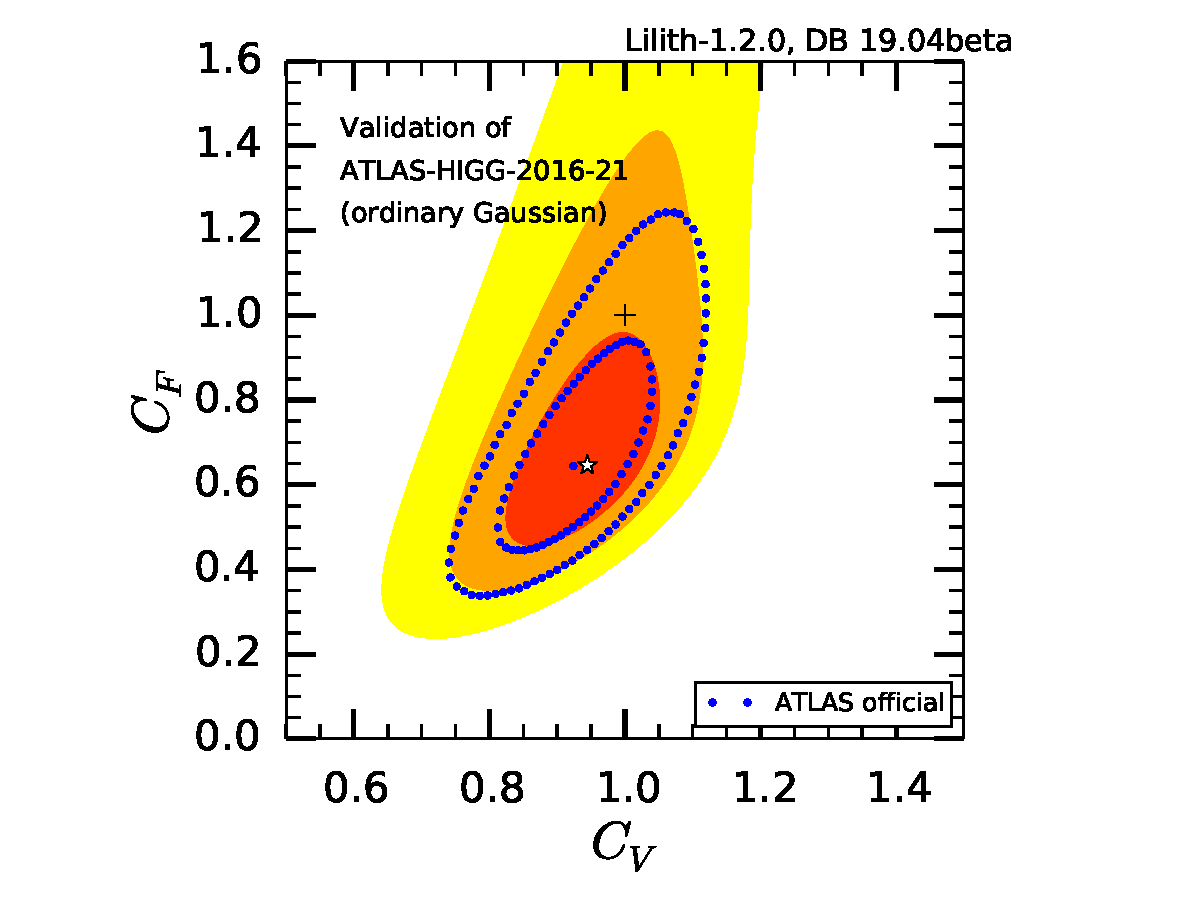
\includegraphics[width=0.43\textwidth]{validation/ATLAS/HIGG-2016-21-CVCF-Gaussian.pdf}%
%\hspace*{-12mm}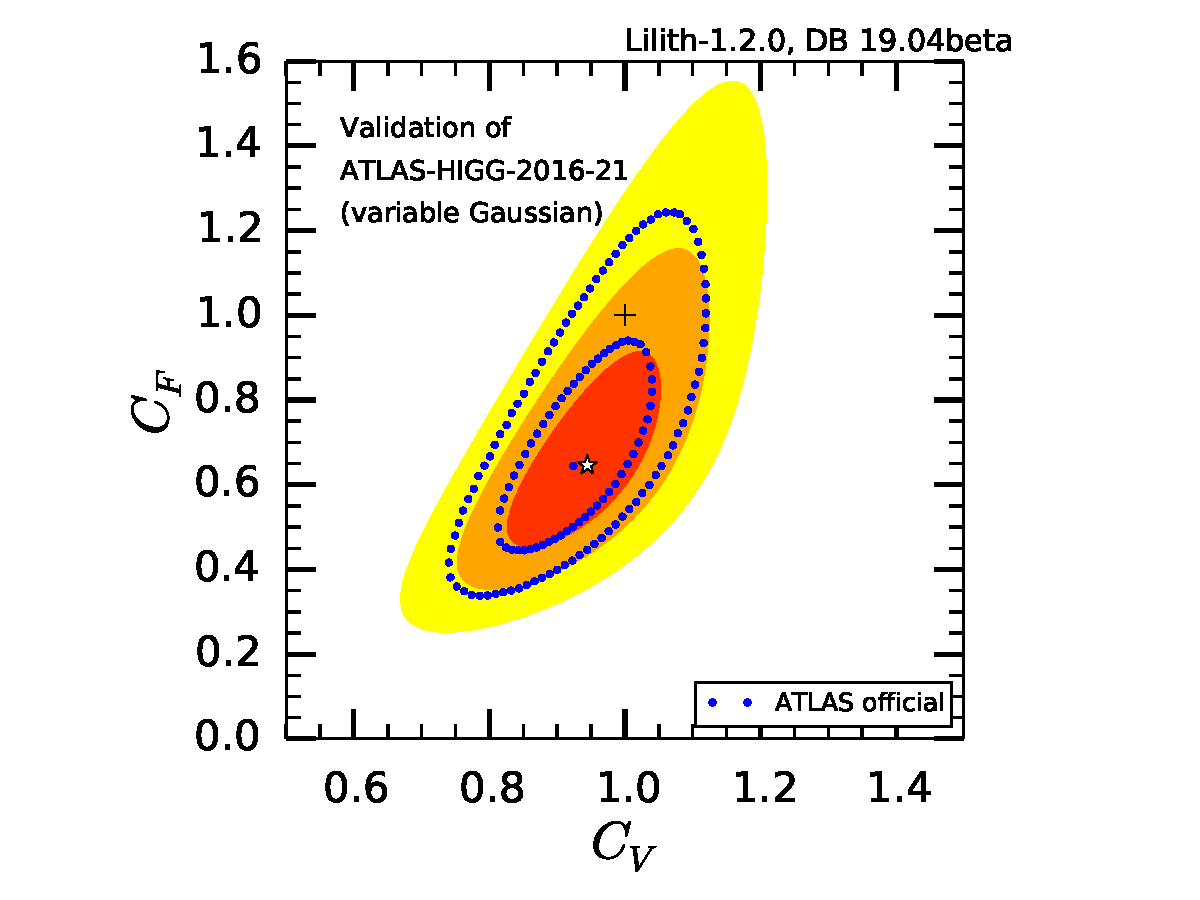
\includegraphics[width=0.43\textwidth]{validation/ATLAS/HIGG-2016-21-CVCF-GaussianV2.pdf}%
%\hspace*{-12mm}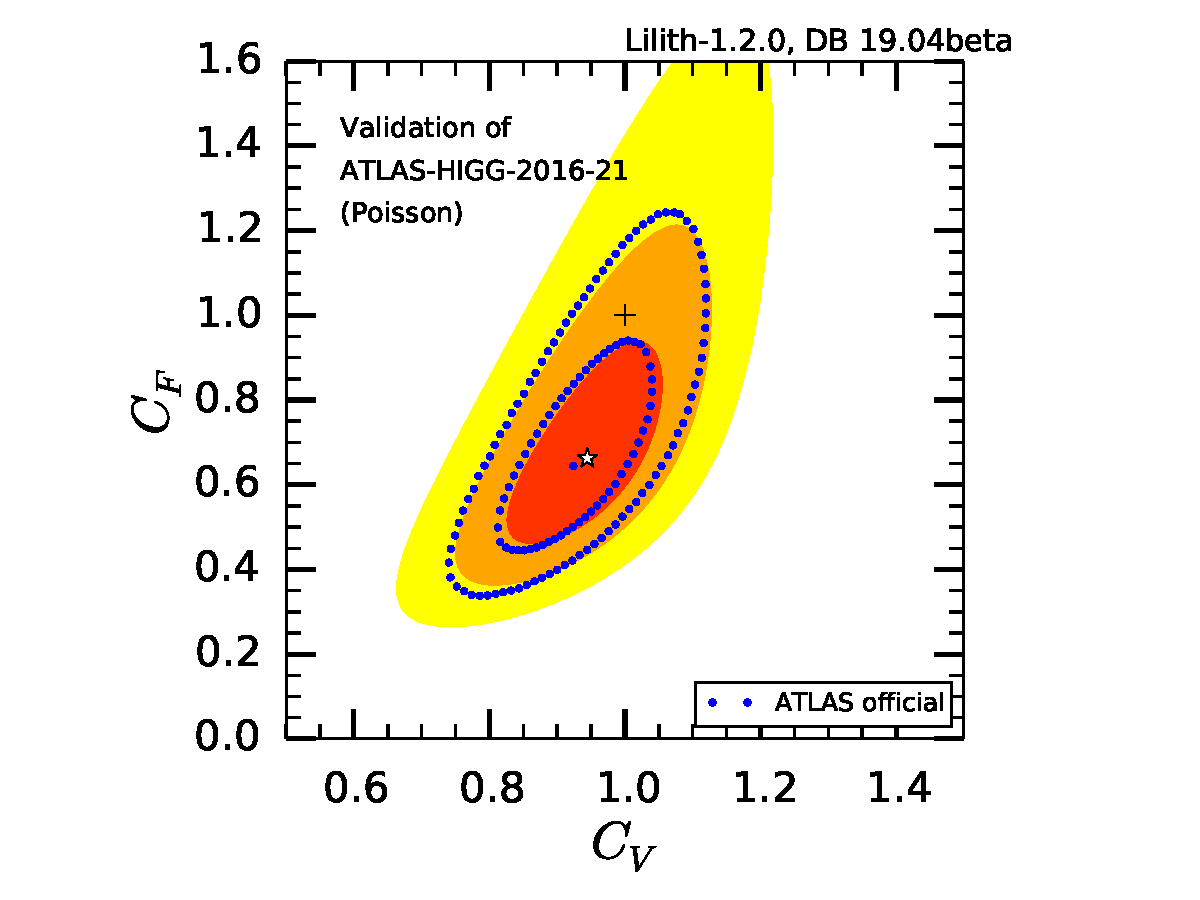
\includegraphics[width=0.43\textwidth]{validation/ATLAS/HIGG-2016-21-CVCF-Poisson.pdf} 
%\caption{Fits of $C_V$ vs.\ $C_F$ using data from the ATLAS $H\to\gamma\gamma$ measurement~\cite{Aaboud:2018xdt}; 
%the signal strength measurements are implemented, from left to right, as ordinary Gaussian, variable Gaussian and Poisson likelihoods.}
%\label{validation_atlas_gamgam}
%\end{figure}
 
{\bf\boldmath $H\to ZZ^*\to 4l$ ( HIGG-2016-22):} \\


{\bf\boldmath $H\to WW^*\to 2l2\nu$ (HIGG-2016-07):} \\

{\bf\boldmath $H\to \tau\tau$ (HIGG-2017-07):} \\

{\bf\boldmath $H\to b\bar b$ (HIGG-2016-29 and HIGG-2016-30):}\\



{\bf\boldmath $H\to$~invisible (HIGG-2016-28):}
Results from the search for invisibly decaying Higgs bosons produced in association with a $Z$ boson are presented in \cite{Aaboud:2017bja}. Assuming the Standard Model $ZH$ production cross-section, an observed (expected) upper limit of 67\% (39\%) at the 95\% confidence level is set on BR$(H\to inv)$ for $m_H= 125$~GeV. We use $1-{\rm CLs}$ as function BR$(H\to inv)$ extracted from auxiliary Figure~1c on the analysis' webpage. 


\clearpage
%-----------------------------------------------------------------------------------------------
\subsection{CMS Run~2 results for 36~fb$^{-1}$}
%-----------------------------------------------------------------------------------------------

The CMS Run~2 results included in this release are summarised in Table~\ref{tab:CMSresults} and explained in more detail below.

\begin{table}[h]\centering
\begin{tabular}{l | ccccccc}
mode & $\gamma\gamma$ & $ZZ$ & $WW$ & $\tau\tau$ & $b\bar b$ & $\mu\mu$ & inv. \\
\hline
ggH & \cite{Sirunyan:2018koj} & \cite{Sirunyan:2018koj} & \cite{Sirunyan:2018koj} & \cite{Sirunyan:2018koj} & \cite{Sirunyan:2018koj} & \cite{Sirunyan:2018koj} & \cite{Sirunyan:2018owy} \\
VBF &  \cite{Sirunyan:2018koj} & \cite{Sirunyan:2018koj} & \cite{Sirunyan:2018koj} & \cite{Sirunyan:2018koj} &-- & \cite{Sirunyan:2018koj} & \cite{Sirunyan:2018owy} \\
WH &  \cite{Sirunyan:2018koj} & \cite{Sirunyan:2018koj} & \cite{Sirunyan:2018koj} & \cite{Sirunyan:2018cpi} & \cite{Sirunyan:2018koj} & -- & \cite{Sirunyan:2018owy} \\
ZH & \cite{Sirunyan:2018koj} & \cite{Sirunyan:2018koj} & \cite{Sirunyan:2018koj} & \cite{Sirunyan:2018cpi} & \cite{Sirunyan:2018koj} & -- & \cite{Sirunyan:2018owy} \\
ttH & \cite{Sirunyan:2018koj} & \cite{Sirunyan:2018koj} & \cite{Sirunyan:2018koj} & \cite{Sirunyan:2018koj} & \cite{Sirunyan:2018koj} & -- & -- \\
\end{tabular}
\caption{Overview of CMS Run~2 results included in this release. Note that we use the full $24\times 24$ correlation matrix 
for the signal strengths for each production and decay mode combination provided in \cite{Sirunyan:2018koj}.}
\label{tab:CMSresults}
\end{table}


{\bf\boldmath Combined measurements (HIG-17-031):} 
CMS presented in \cite{Sirunyan:2018koj} a combination of the individual measurements for the 
$H\to \gamma\gamma$~\cite{Sirunyan:2018ouh}, $ZZ$~\cite{Sirunyan:2017exp}, $WW$~\cite{Sirunyan:2018egh}, 
$\tau\tau$~\cite{Sirunyan:2017khh}, $b\bar b$~\cite{Sirunyan:2017elk,Sirunyan:2017dgc} and $\mu\mu$~\cite{Sirunyan:2018hbu} 
decay modes as well as the $t\bar tH$ analyses~\cite{Sirunyan:2018shy,Sirunyan:2018mvw,Sirunyan:2018ygk}. 
We use the best fit values and uncertainties for the signal strengths for each production %(ggH, VBF, WH, ZH, ttH) 
and decay  %($\gamma\gamma$, $ZZ$, $WW$, $\tau\tau$, $b\bar b$, $\mu\mu$) 
mode combination presented in Table~3 of \cite{Sirunyan:2018koj} together with the $24\times 24$ correlation matrix 
provided as ``Additional Figure~1'' on the analysis webpage. As shown in Fig.~\ref{fig:validation_cms_combination}, 
this allows to reproduce well the coupling fits of the CMS paper.\\

\begin{figure}[t!]\centering
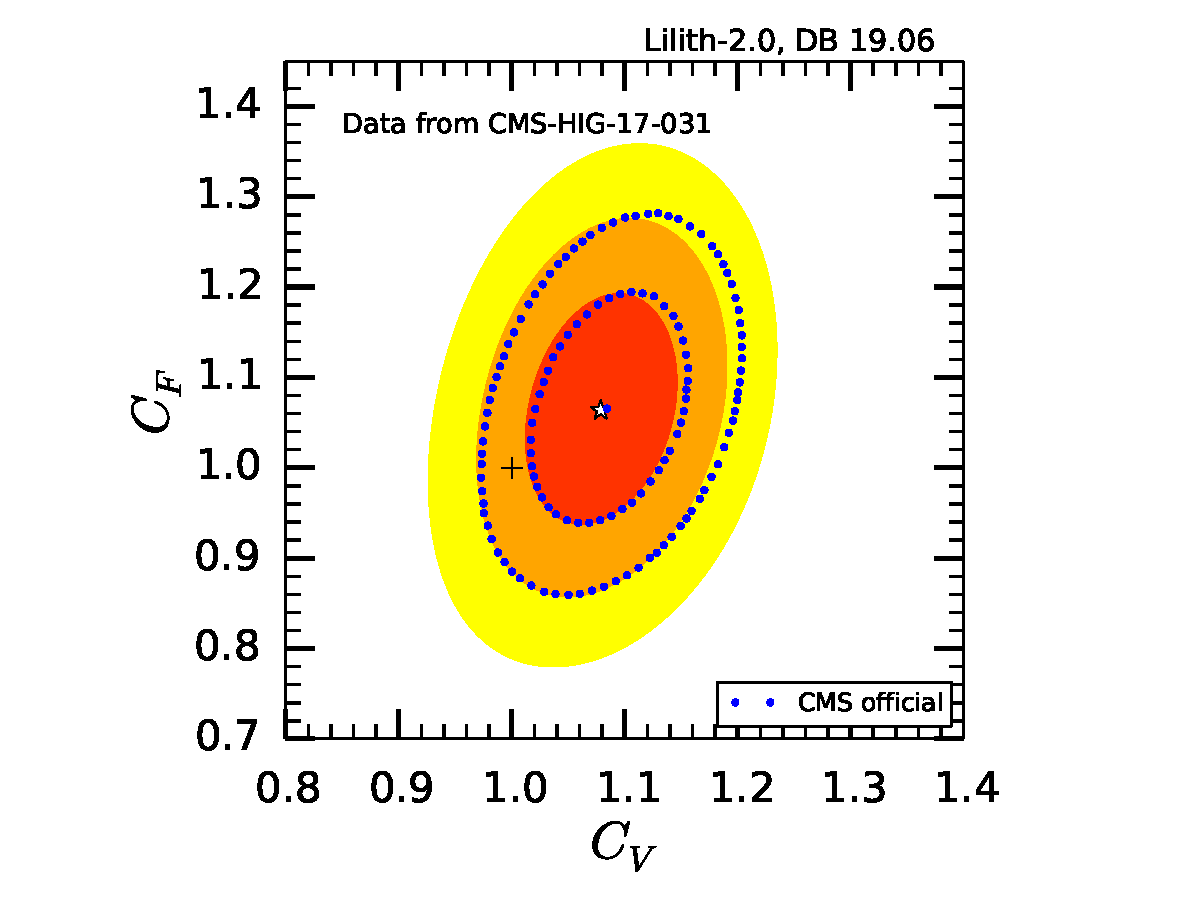
\includegraphics[width=0.5\textwidth]{validation/CMS/HIG-17-031-CVCF.pdf}
\caption{Fit of $C_F$ vs.\ $C_V$ using best fit values and uncertainties for the signal strengths for each production (ggH, VBF, WH, ZH, ttH) 
and decay ($\gamma\gamma$, $ZZ$, $WW$, $\tau\tau$, $b\bar b$, $\mu\mu$) mode combination together with the 
$24\times 24$ correlation matrix from the CMS combination paper~\cite{Sirunyan:2018koj}. 
The  $1\sigma$,  $2\sigma$ and $3\sigma$ regions obtained with {\tt Lilith} are shown as red, orange and yellow areas, 
and compared to the $1\sigma$ and $2\sigma$ contours from CMS (blue dots).}
\label{fig:validation_cms_combination}
\end{figure}

\begin{figure}[t!]\centering
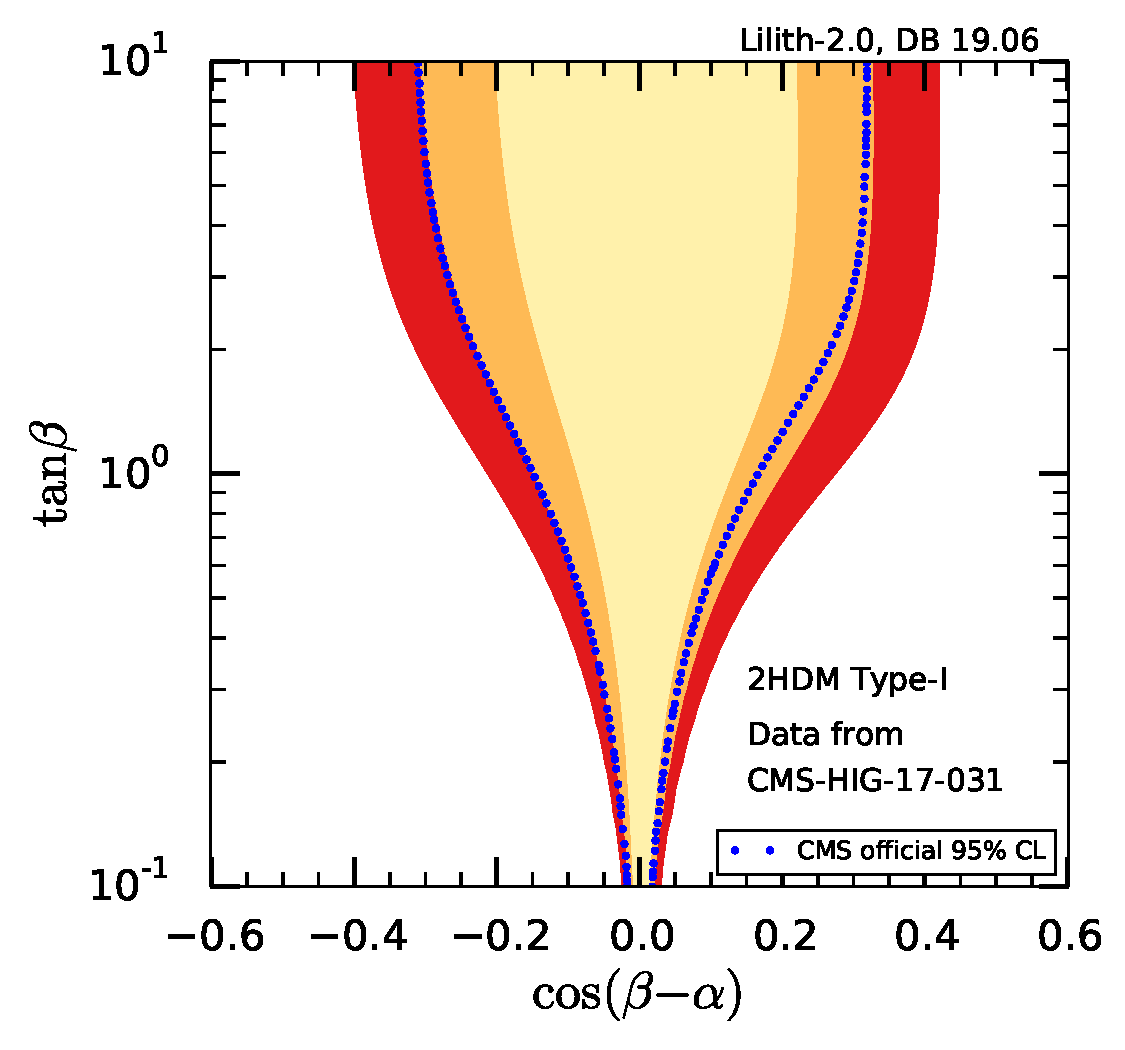
\includegraphics[width=0.4\textwidth]{validation/CMS/HIG-17-031-2HDM-Type1.pdf}%
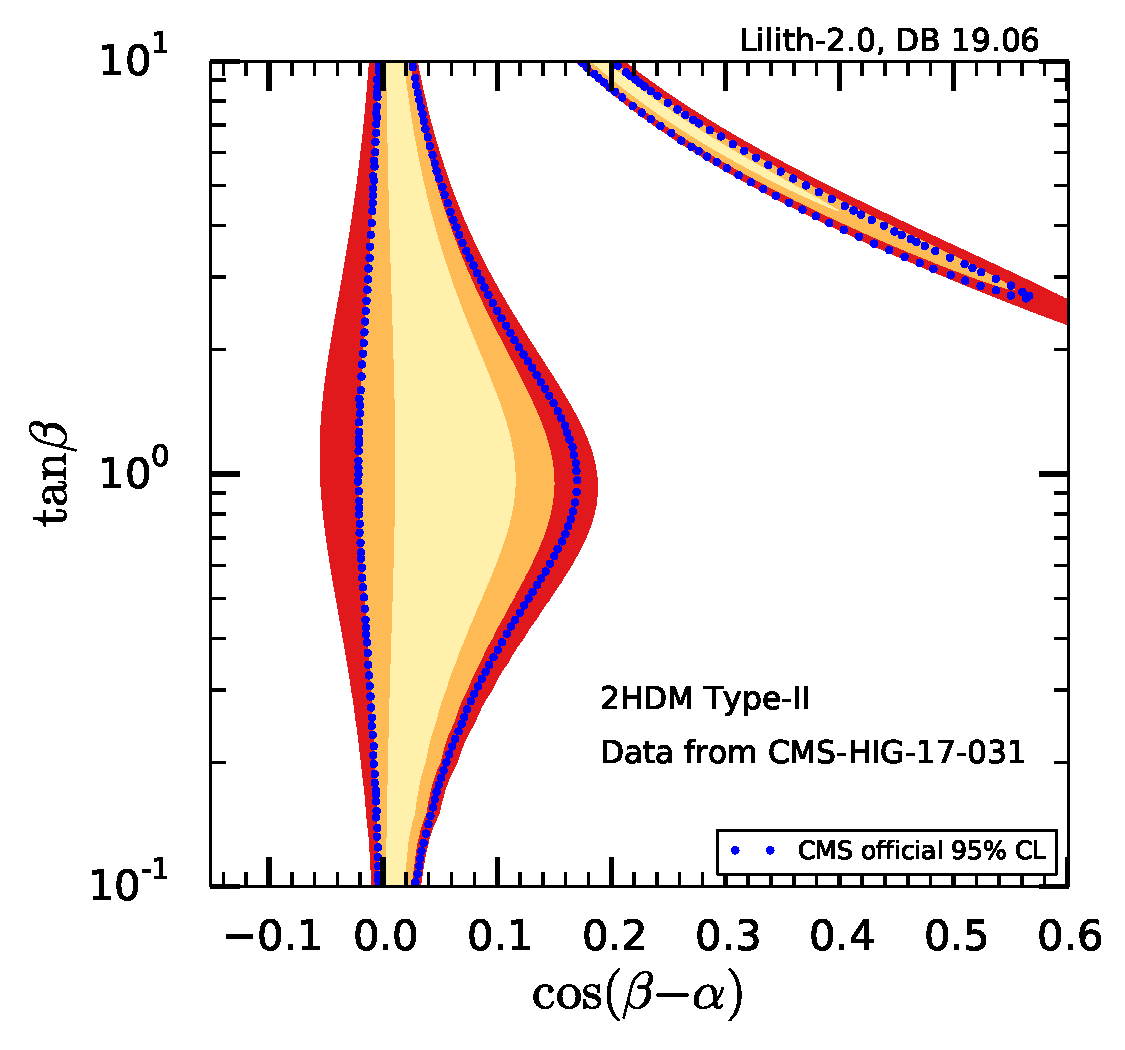
\includegraphics[width=0.4\textwidth]{validation/CMS/HIG-17-031-2HDM-Type2.pdf}
\caption{Fit of $\tan\beta$ vs.\ $\cos(\beta-\alpha)$ for the Two-Higgs-Doublet models of Type~I (left) and Type~II (right) 
using the data from the combined CMS measurement~\cite{Sirunyan:2018koj}. 
The beige, orange and red filled areas show the 68\%, 95\% and 99.7\% CL regions obtained with {\tt Lilith}, 
while the blue dots mark the 95\% CL contours from CMS.}
\label{fig:validation_cms_2hdm}
\end{figure}

{\bf\boldmath $VH$, $H\to\tau\tau$ (HIG-18-007)}: The above data from \cite{Sirunyan:2018koj} is supplemented by the results 
for the $\tau\tau$ decay mode from the $WH$ and $ZH$ targeted analysis \cite{Sirunyan:2018cpi}. These are implemented in the 
form of 1D intervals for $\mu(ZH,\;H\to\tau\tau)$ and $\mu(WH,\;H\to\tau\tau)$ taken from Fig.~6 of \cite{Sirunyan:2018cpi}. \\

{\bf\boldmath $H\to$~invisible (HIG-17-023)}: 
In \cite{Sirunyan:2018owy}, CMS performed a search for invisible decays of a Higgs boson produced through vector boson fusion. 
We use the profile likelihood ratios for the qqH-tag, Z(ll)H-, V(qq')H- and ggH-tag categories extracted 
from their Fig.~8b together with the relative contributions from the different Higgs production mechanisms  
given in Table~6 of that paper. This assumes that the relative signal contributions stay roughly the same as for 
SM production cross sections. For validation, we reproduce in Fig.~\ref{fig:validation_cms_inv}
 the $C_g$ vs.\ $C_\gamma$ fit of \cite{Sirunyan:2018koj}, where the branching ratios of invisible and undetected decays 
are treated as free parameters.\footnote{The profiling was done with {\tt Minuit}. Since {\tt Minuit} does not allow conditional limits, in this case 
${\rm BR}(H\to {\rm inv.})+{\rm BR}(H\to {\rm undetected})<1$, we demanded that both BR$(H\to {\rm inv.})$ and BR$(H\to {\rm undetected})$ 
be less than 50\%.} 

\begin{figure}[t!]\centering
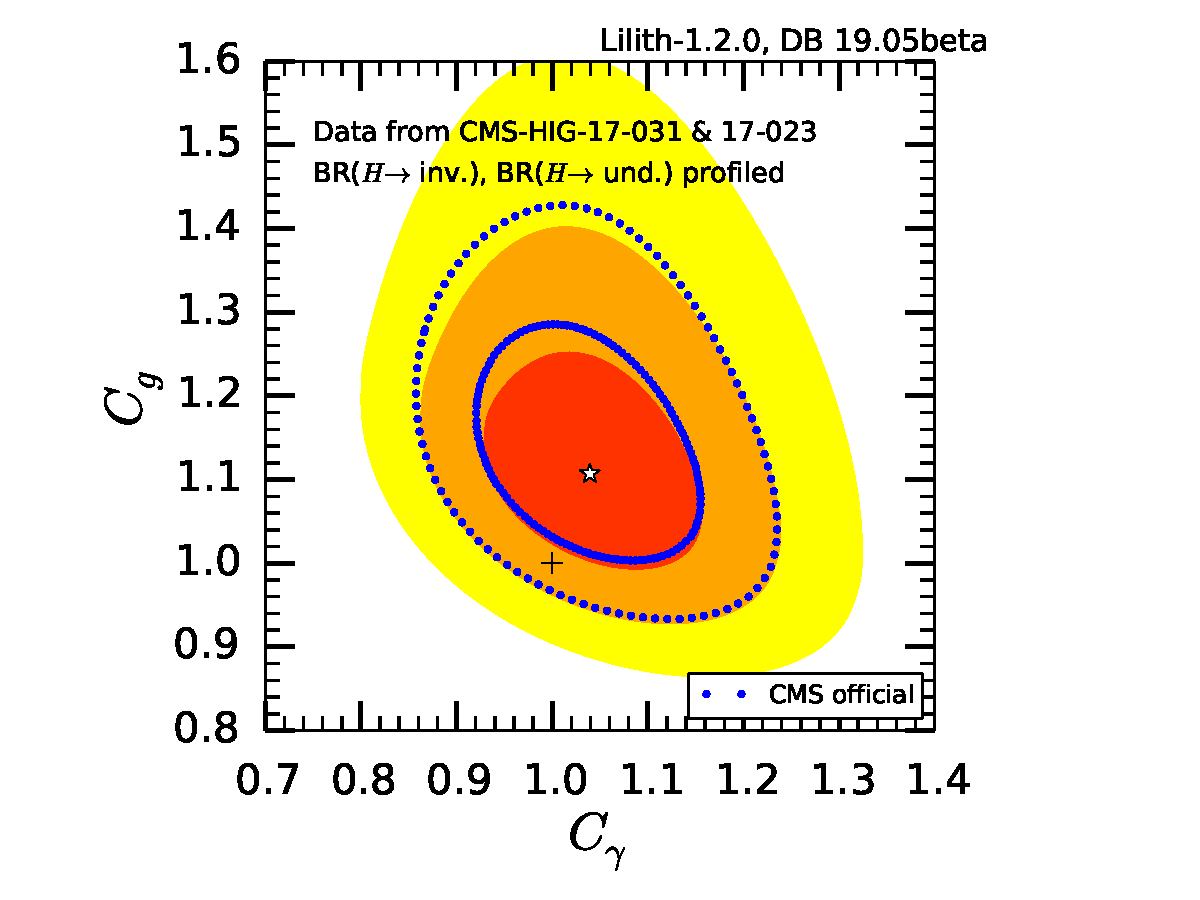
\includegraphics[width=0.5\textwidth]{validation/CMS/HIG-17-031-CgCGa_BRinvBRund_profiled.pdf}
\caption{Fit of $C_g$ vs.\ $C_\gamma$ using the data from the combined CMS measurement~\cite{Sirunyan:2018koj} and the 
search for invisible decays of a Higgs boson~\cite{Sirunyan:2018owy}. The branching ratios of invisible and undetected decays 
are treated as free parameters in the fit. 
The  $1\sigma$,  $2\sigma$ and $3\sigma$ regions obtained with {\tt Lilith} are shown as red, orange and yellow areas, 
and compared to the $1\sigma$ and $2\sigma$ contours from CMS (in blue).}
\label{fig:validation_cms_inv}
\end{figure}




%===================================================================================
\section{Status of Higgs coupling fits}
%===================================================================================


%===================================================================================
\section{Conclusion}
%===================================================================================
 must include a conclusion.

%===================================================================================
\section*{Acknowledgements}
%===================================================================================

S.K.~thanks W.~Adam, R.~Sch\"ofbeck, W.~Waltenberger and N.~Wardle for helpful discussions. 
This work was supported in part by the IN2P3 theory project 
``LHC-itools: methods and tools for the interpretation of the LHC Run~2 results for new physics''. 
D.T.N.\ thanks the LPSC Grenoble for hospitality and financial support for a research visit within the LHC-itools project. 
L.T.Q.\ thanks the ICISE ...


%===================================================================================
\begin{appendix}
%===================================================================================

\section{Overview of XML data files}

\section{Implementation of 2D Poisson likelihood with correlation}
\subsection{Log-likelihood for Poisson distribution with continuous variable}
The probability mass function of Poisson distribution, with parameter $\lambda>0$, and variable $k = 0,1,2,3, ...$:
\begin{align}
f(k; \lambda)= \frac{e^{-\lambda}\lambda^k}{k!}.
\end{align}
The log-likelihood function for Poisson distribution:
\begin{align}
l(\lambda; k) = \log [f(k;\lambda)]=-\lambda + k\log \lambda - \log k!. \label{P_llh}
\end{align}
Here, since $k$ is a discrete variable, we would redefine a log-likelihood function of parameter $\lambda$ that fix continuous variable, denoted as ``$\nu$". We re-define the parameter as $\lambda \equiv \rho(\lambda-c)+ \tau$, with $\eta = {\tau}/{\rho}$, and $c$ is the expected value at which the log-likelihood function reaches extrema. The new log-likelihood function reads:
\begin{align}
l(\lambda;\nu)&=-\rho(\lambda-c+\eta)+\nu\log\rho(\lambda-c+\eta)+\text{const}.
\end{align}
Here we want to set the extrema at $\lambda=c$. Since the Poisson distribution has expected value equal it parameter, we set $\nu = \rho\eta$ so that the log-likelihood function reaches extrema at $f(c)$. For Poisson distribution, the extrema of log-likelihood function is not equal 0, we will consider its $\Delta$ log-likelihood function:
\begin{align}
\Delta l(\lambda;\nu)=l(\lambda;\nu)-l(c;\nu)=	-\rho (\lambda-c)+\nu\ln\left[1+\frac{\rho}{\nu}( \lambda-c)\right].\label{P_delta_llh}
\end{align}
$\Delta l(\sigma_-;\nu)$ and $\Delta l(\sigma_+;\nu)$ yields $-1/2$, dividing their r.h.s terms of by $\nu$ followed by taking the exponentials, we get the relation:
\begin{align}
\frac{1-\gamma\sigma_-}{1-\gamma\sigma_+}=e^{-\gamma(\sigma_-+\sigma_+)}.
\end{align}
From $\Delta l(\sigma_+;\nu) = -1/2$, we could derive $\nu$:
\begin{align}
\nu=\frac{1}{2(\gamma\sigma_+-\ln(1+\gamma\sigma_+))}.
\end{align}
\subsection{A model for bivariate Poisson distribution with negative correlation}
For references, see: \hyperlink{http://www.economists.nl/files/20130411-SN2004.pdf}{Berkhout, Plug's}.\\
The probability mass function (pmf) of Poisson distribution, with parameter $\lambda>0$, and variable $k = 0,1,2,3, ...$:
\begin{align}
f(k; \lambda)= \frac{e^{-\lambda}\lambda^k}{k!}.
\end{align}
We would like to apply a model of bivariate Poisson distribution which allows negative correlation. We define marginal and dependent pmf respectively as:
\begin{align}
g_{1}(k_{1};\lambda_1)=\frac{e^{-\lambda_{1}}\lambda_{1}^{k_{1}}}{k_{1}!},\\g_{2}(k_{2}|k_{1};\lambda_2)=\frac{e^{-\lambda_{2}}\lambda_{2}^{k_{2}}}{k_{2}!}.
\end{align}
By convention, the parameters read:
\begin{align}
\lambda_1&= e^{x'\beta_1},\\\lambda_2&=e^{x'\beta_2+\alpha k_1}.
\end{align}
The parameter $\alpha$ is added as a small correction that correspondent for the correlation of $k_1,k_2$. The joint pmf:
\begin{align}
f(k_1,k_2;\lambda_1,\lambda_2)=g_2(k_2|k_1;\lambda_2)g_1(k_1;\lambda_1). 
\end{align}
The marginal pmf remains the form of Poisson distribution, its expected value and variance reads:
\begin{align}
E(k_1)=\text{Var}(k_1)=\lambda_1.
\end{align}
The (r, s)th factorial moment of the joint distribution is derived as:
\begin{align}
&E\left[k_1(k_1-1)...(k_1-r+1)k_2(k_2-1)...(k_2-s+1)\right]\\=&\sum^{\infty}_{k_1=r}\sum^{\infty}_{k_2=s}\frac{e^{k_1(x'\beta_1)-\exp(x'\beta_1)+k_2(x'\beta_2+\alpha k_1)-\exp(x'\beta_2+\alpha k_1)}}{(k_1-r)!(k_2-s)!}\\=&\lambda_1^re^{\lambda_1[\exp(s\alpha)-1]+sx'\beta_2+rs\alpha}.\label{moment}
\end{align}
The expected value, variance of $k_2$ and expected value of $k_1k_2$ is derived from the factorial moment \ref{moment} as:
\begin{align}
&E(k_2)=e^{x'\beta_2+(\exp(\alpha)-1)\lambda_1},\\
&\text{Var}(k_2)=E(k_2)+[E(k_2)]^2\{e^{\lambda_1[\exp(\alpha)-1]}\},\\&E(k_1k_2)=\lambda_1E(k_2)\exp(\alpha).
\end{align}
The covariance of $k_1$ and $k_2$ reads:
\begin{align}
\text{Cov}(k_1,k_2)=E(k_1k_2)-E(k_1)E(k_2)=\lambda_1E(k_2)[\exp(\alpha)-1].
\end{align}
The correlation reads:
\begin{align}
\text{Corr}(k_1,k_2) = \frac{\lambda_1E(k_2)[\exp(\alpha)-1]}{\sqrt{\lambda_1E(k_2)\{1+E(k_2)\{e^{\lambda_1[\exp(\alpha)-1]^2}-1\}\}}}.\label{Corr}
\end{align}
For later convenience, we derive the relation between $\lambda_2$ and $E(k_2)$:
\begin{align}
\lambda_2 = E(k_2)e^{\alpha k_1 - [\exp(\alpha)-1]\lambda_1}=E(k_2)e^{\alpha k_1 - [\exp(\alpha)-1]E(k_1)}.\label{relation}
\end{align}
\subsection{Log-likelihood for bivariate Poisson distribution with continuous variable and negative correlation}
We derive a log-likelihood function that fixes continuous variables for the bivariate Poisson distribution which allows negative correlation. Now for the marginal pmf:
\begin{align}
g_{1}(k_{1};\lambda_1)=\frac{e^{-\lambda_{1}}\lambda_{1}^{k_{1}}}{k_{1}!}.
\end{align}
It remains the form of ordinary Poisson distribution. We apply \ref{P_delta_llh} to derive the $\Delta$ log-likelihood function:
\begin{align}
\Delta l_1(\lambda_1;\nu_1) = -\rho_1(\lambda_1-c_{1}) + \nu_1\log\left[1+\frac{\rho_1}{\nu_1}(\lambda_1-c_1)\right].
\end{align}
Considering the dependent pmf:
\begin{align}
g_{2}(k_{2}|k_{1};\lambda_2)=\frac{e^{-\lambda_{2}}\lambda_{2}^{k_{2}}}{k_{2}!}.
\end{align}   
Its log-likelihood function fixing discrete variable $k_2$:
\begin{align}
l_2(\lambda_2; k_2) = \log [g_{2}(k_{2}|k_{1};\lambda_2)]=-\lambda_2 + k_2\log \lambda_2 - \log k_2!,
\end{align}
with the parameter $\lambda_2$ reads:
\begin{align}
\lambda_2 = E(k_2)e^{\alpha k_1 - [\exp(\alpha)-1]E(k_1)}.
\end{align}
For fixing continuous variable $\nu_2$, we redefine the parameter $\lambda_2$ as:
\begin{align}
\lambda_2 \equiv \rho_2(\lambda_2 - c_2 + \eta_2)e^{\alpha \nu_1 - [\exp(\alpha)-1]\rho_1(\lambda_1-c_1+\eta_1)}.
\end{align}
The log-likelihood function $l_2$ now become a function of two parameters $\lambda_1, \lambda_2$ fixing two variables $\nu_1, \nu_2$:
\begin{align}
l_2(\lambda_1,\lambda_2; \nu_1,\nu_2) =-\lambda_2 + \nu_2\log \lambda_2 + \text{const}.
\end{align}
Its $\Delta$ log-likelihood function reads:
\begin{align}
\Delta l_2(\lambda_1,\lambda_2; \nu_1,\nu_2)=l_2(\lambda_1,\lambda_2; \nu_1,\nu_2)-l_2(c_1,c_2; \nu_1,\nu_2).
\end{align}
The correlation in \ref{Corr} becomes: 
\begin{align}
\text{Corr}(\nu_1,\nu_2) = \frac{\nu_1\nu_2[\exp(\alpha)-1]}{\sqrt{\nu_1\nu_2\{1+\nu_2\{e^{\nu_1[\exp(\alpha)-1]^2}-1\}\}}}.
\end{align}
Finally, the $\Delta$log-likelihood for joint pmf:
\begin{align}
\Delta l_{\text{join}}(\lambda_1,\lambda_2;\nu_1,\nu_2)=\Delta l_1(\lambda_1;\nu_1) + \Delta l_2(\lambda_1,\lambda_2; \nu_1,\nu_2).
\end{align}
\end{appendix}


%===================================================================================
% References
%===================================================================================

% \bibliographystyle{SciPost_bibstyle} % Include this style file here only if you are not using our template
\bibliography{references.bib}

\nolinenumbers

\end{document}
